
\section{Activity diagram giữa hệ thống và các bên liên quan trong Task Assignment Module}
    \begin{figure}[h]
        \centering
        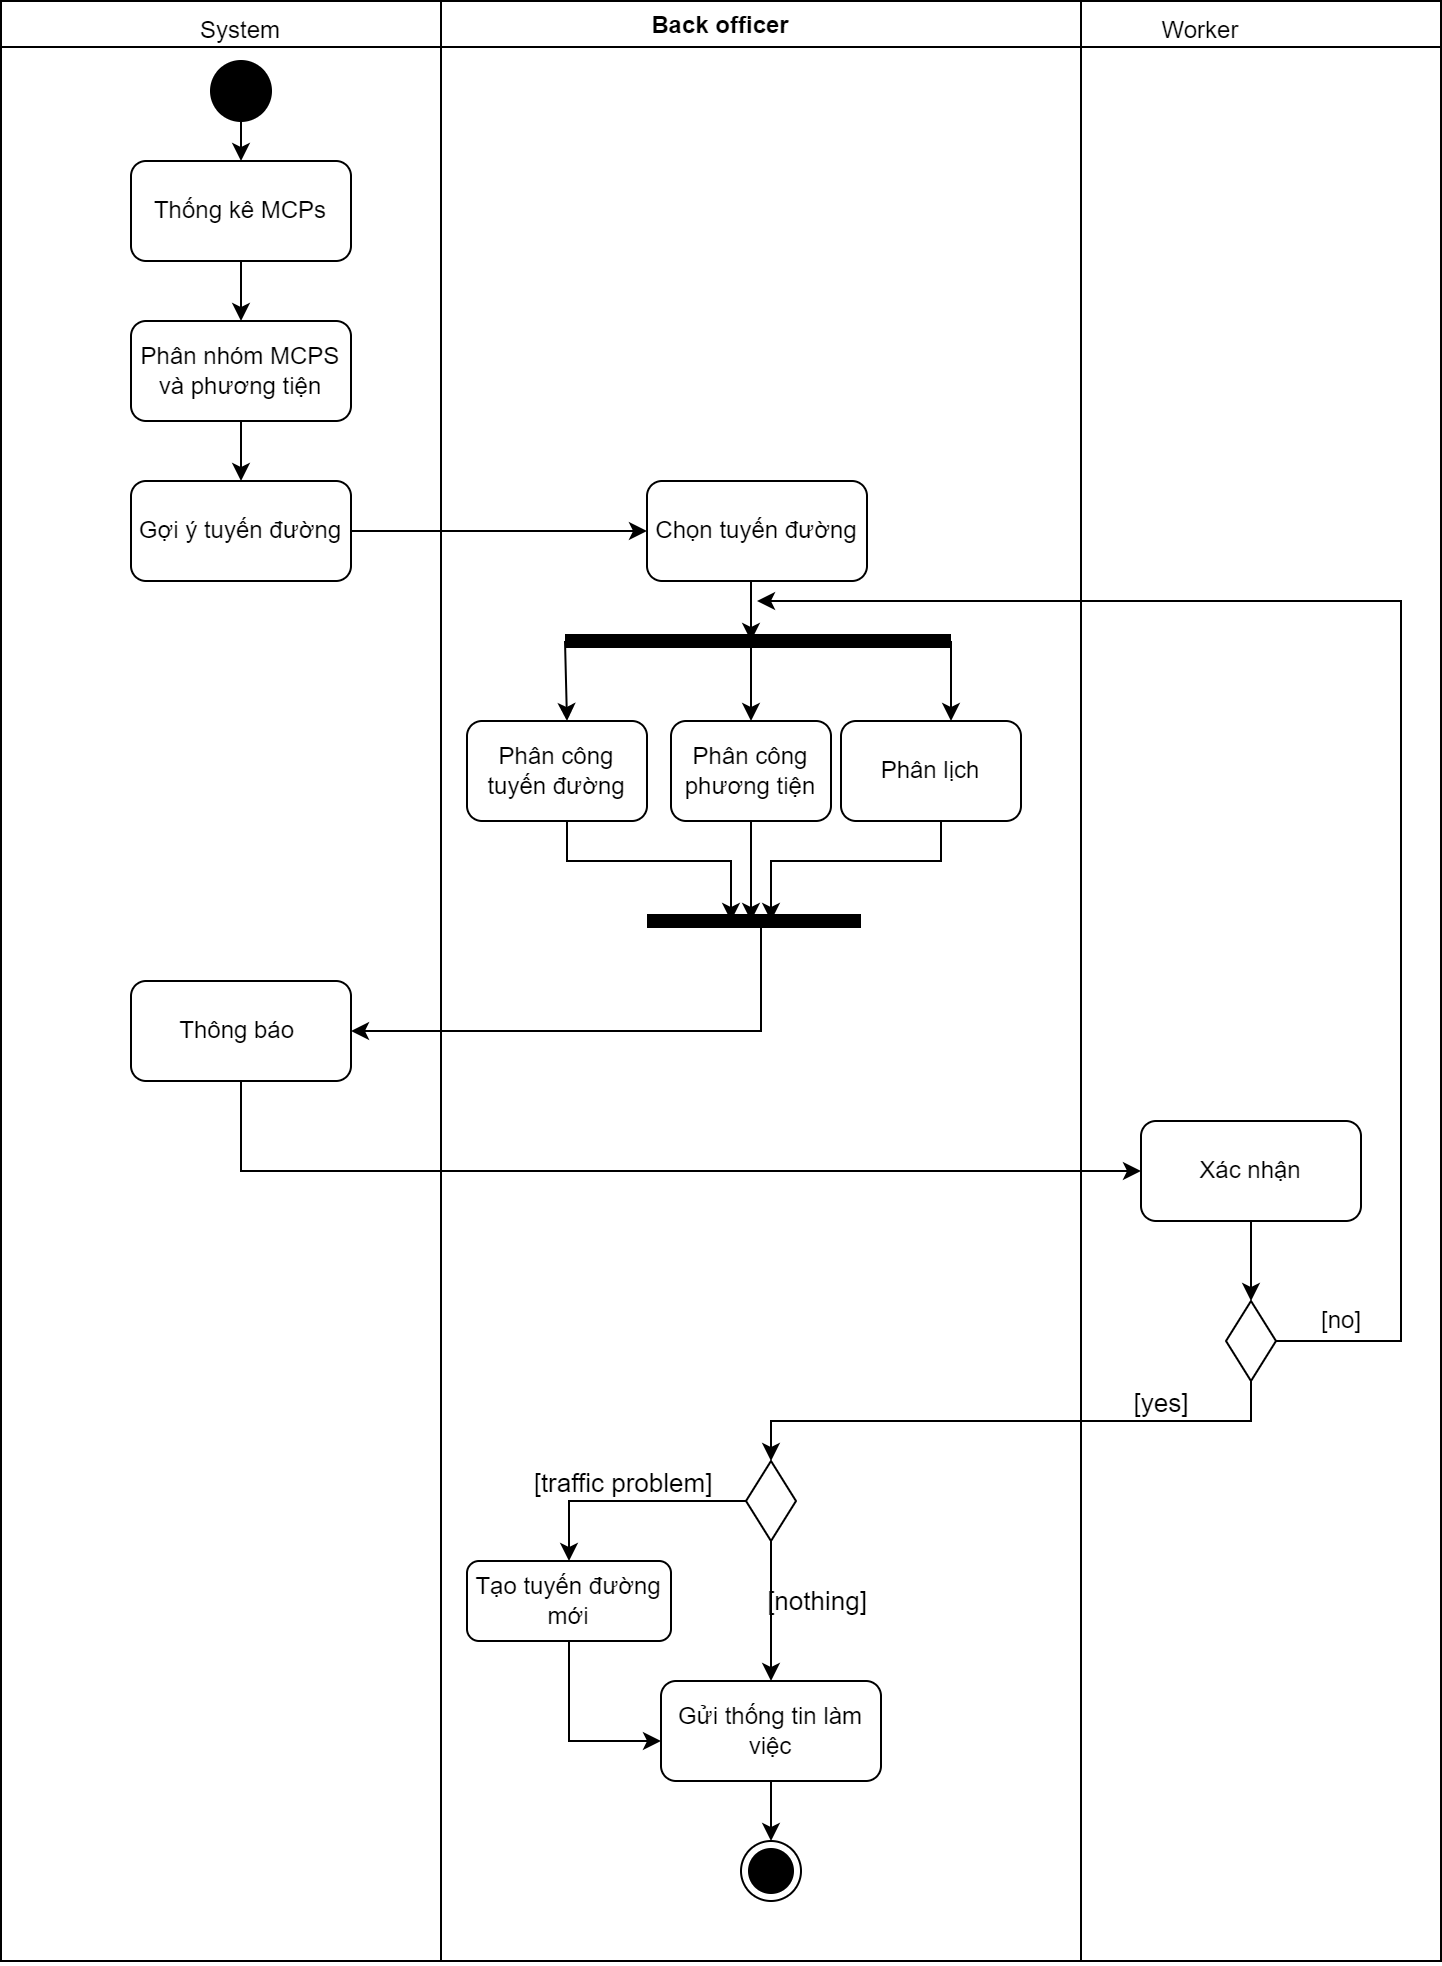
\includegraphics[width=15.0cm,height=15cm]{imgs/activity diagram/activity diagram.png}
        \caption{Activity diagram trong Task Asssignment Module}
    \end{figure}
    \newpage
    Hoạt động giữa hệ thống và các bên liên quan trong Task Assignment Module gồm các hoạt động theo thứ tự:
    \begin{enumerate}
        \item Bắt đầu.
        \item Hệ thống thống kê số lượng, vị trí MCPs.
        \item Hệ thống phân nhóm MCPs theo vùng phù hợp với sức chứa của phương tiện hiện có để tối ưu về tuyến đường và nhiên liệu.
        \item Hệ thống gợi ý các tuyến đường tối ưu cho Back officer.
        \item Back officer chọn tuyến đường cho tháng.
        \item Back officer phân công tuyến đường, phân phương tiện và tạo lịch cho collectors, janitors.
        \item Hệ thống gửi thông báo cho collectors, janitors.
        \item  Collectors, janitors xem thông báo được gửi.
        \item Back officer gửi thông tin làm việc theo ngày cho collectors, janitors.
        \item Kết thúc
    \end{enumerate}
